% Authors: Nelson Lago and Fernanda Magano
% This file is distributed under the MIT Licence

%%%%%%%%%%%%%%%%%%%%%%%%%%%%%%%%%%%%%%%%%%%%%%%%%%%%%%%%%%%%%%%%%%%%%%%%%%%%%%%%
%%%%%%%%%%%%%%%%%%%%%%%%%%%%%%%%% PREÂMBULO %%%%%%%%%%%%%%%%%%%%%%%%%%%%%%%%%%%%
%%%%%%%%%%%%%%%%%%%%%%%%%%%%%%%%%%%%%%%%%%%%%%%%%%%%%%%%%%%%%%%%%%%%%%%%%%%%%%%%

% aspectratio default é 4:3;
% as mais úteis são 169 (16:9), 1610 (16:10) e 149 (14:9)
% A língua padrão é a última citada
\documentclass[xcolor={usenames,svgnames,dvipsnames},brazil,english,12pt,aspectratio=149]{beamer}

% Funções auxiliares essenciais
\usepackage{etoolbox}
\usepackage{xstring}
\usepackage{xparse}
\usepackage{diagbox}
\usepackage{pifont}

% Vários pacotes e opções de configuração genéricos
\input{extras/basics}
% A fonte precisa ser definida depois que o tema metropolis foi carregado
%\input{extras/fonts}
\input{extras/floats}
% index não é necessário, mas deixamos aqui para usar os mesmos
% passos de compilação que a tese
\input{extras/index}
\input{extras/hyperlinks}
\input{extras/source-code}
\input{extras/utils}

% Diretório onde estão as figuras; com isso, não é preciso colocar o caminho
% completo em \includegraphics (e nem a extensão).
\graphicspath{{figuras/}}

% Comandos rápidos para mudar de língua:
% \en -> muda para o inglês
% \br -> muda para o português
% \texten{blah} -> o texto "blah" é em inglês
% \textbr{blah} -> o texto "blah" é em português
\babeltags{br = brazil, en = english}


%%%%%%%%%%%%%%%%%%%%%%%%%%%% APARÊNCIA DO BEAMER %%%%%%%%%%%%%%%%%%%%%%%%%%%%%%%

\usepackage{appendixnumberbeamer}

% Tema metropolis com algumas modificações
\dowithsubdir{extras/}{\usetheme{imeusp}}

% O padrão usa um tom de vermelho escuro como cor principal; a opção
% "greeny" troca essa cor por um tom de verde; a opção "sandy" usa o
% mesmo tom de verde mas modifica a cor padrão dos blocos para um
% tom amarelado.
\dowithsubdir{extras/}{\usecolortheme[abstract2concrete]{siqueira}}
% Desabilita a cor de rodapé
\setbeamercolor{footline}{fg=,bg=}

%%%%%%%%%%%%%%%%%%%%%%%%%% COMANDOS PARA O USUÁRIO %%%%%%%%%%%%%%%%%%%%%%%%%%%%%

\newcommand\col{\column{.5\textwidth}}

% A cada nova seção, recapitula o sumário
% Para desabilitar, é só comentar este trecho
%\AtBeginSection[]{
%  \begin{frame}<beamer>{Overview}
%    \intermezzo
%  \end{frame}
%}

\AtBeginSection[]{}

% Blocos de cor personalizada
\newenvironment{coloredblock}[2]%
{
    \setbeamercolor{block title}{fg=white,white}
    \setbeamercolor{block body}{fg=white,white}
    \setbeamercolor{local structure}{fg=white,bg=white}
    \begin{block}{#2}
}{
    \end{block}
}

%%%%%%%%%%%%%%%%%%%%%%%%%%%%%%%%% METADADOS %%%%%%%%%%%%%%%%%%%%%%%%%%%%%%%%%%%%

% Referências
\usepackage[style=bwl-FU]{biblatex}
\addbibresource{bibliografia.bib}
% Acrescenta à lista de referências sem precisar incluir uma referência
% de fato no texto
\nocite{bronevetsky02,schmidt03:MSc, FSF:GNU-GPL, CORBA:spec, MenaChalco08}
% Acrescenta tudo do arquivo .bib
%\nocite{*}
\title[The shortened title]{Uma Visão Sobre a Próxima Geração de Abstrações de Processos em Sistemas Operacionais}
%\subtitle{The (optional) subtitle}

\author[Rodrigo Siqueira Jordão]{Rodrigo Siqueira Jordão}

\institute[USP]{\textbf{Orientador: Fabio Kon} \\ Instituto de Matemática e Estatística \\ IME USP}
%\institute[USP]{\textbf{Orientador:} \\ Computer Science Department \\ IME USP}

%\date{Month and day, year}

% Coloca a imagem no fundo da página de título
%\bgimage{\includegraphics[width=\paperwidth]{fundo_predios_e_grafo}}

% Logotipos no rodapé da página de título
\logos{
  \hfil\hfil\includegraphics[width=.1\textwidth]{usp-logo}\hfil%
  \raisebox{-.0103\paperheight}{\includegraphics[height=.0932\paperheight]{interscity-logo-branco}}\hfil%
%  \raisebox{-.00517\paperheight}{\includegraphics[height=.057\paperheight]{cnpq-logo}}\hfil%
  \raisebox{-.033\paperheight}{\includegraphics[width=.07\textwidth,trim=0 230 0 0,clip]{ime-logo}}\hfil\hfil
}

%\logos{
%  \hfil\hfil\includegraphics[width=.1\textwidth]{usp-logo}\hfil%
%  \raisebox{-.0103\paperheight}{\includegraphics[height=.0932\paperheight]{interscity-logo}}\hfil%
%  \raisebox{-.00517\paperheight}{\includegraphics[height=.057\paperheight]{cnpq-logo}}\hfil%
%  \raisebox{-.0342\paperheight}{\includegraphics[height=.1035\paperheight]{capes-logo}}\hfil%
%  \includegraphics[height=.044\paperheight]{fapesp-logo}\hfil\hfil
%}

% Usado para criar o qrcode com o endereço da apresentação
\presentationurl{https://siqueira.tech}

% Inclui o qrcode no sumário da apresentação
\includeqrcodeintoc

% O slide de sumário pode ser dividido em colunas; o parâmetro
% determina após qual o número da seção fazer a quebra de coluna
% (use zero para uma coluna ou simplesmente omita este comando).
\toccolumns{4}


%%%%%%%%%%%%%%%%%%%%%%%%%%%%%%%%%%%%%%%%%%%%%%%%%%%%%%%%%%%%%%%%%%%%%%%%%%%%%%%%
%%%%%%%%%%%%%%%%%%%%%%%%%%%% INÍCIO DA APRESENTAÇÃO %%%%%%%%%%%%%%%%%%%%%%%%%%%%
%%%%%%%%%%%%%%%%%%%%%%%%%%%%%%%%%%%%%%%%%%%%%%%%%%%%%%%%%%%%%%%%%%%%%%%%%%%%%%%%

\begin{document}
\definecolor{MyBackground}{rgb}{255, 255, 255}
\setbeamercolor{background canvas}{bg=MyBackground}
\def\apresentacao{\relax}

% É complicado colocar uma imagem de fundo, os logos das agências e
% o conteúdo "normal" do slide de título sem que as coisas fiquem
% bagunçadas, então definimos um comando para gerar o slide de título
\customtitlepage

% Slide com o qrcode
%\showqrcode

\begin{frame}[plain]
  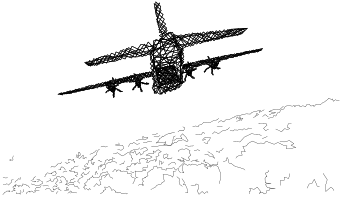
\includegraphics[width=\textwidth]{airplane}
\end{frame}

%------------------------------------------------------------------------------
% FUNDAMENTAÇÃO TEÓRICA
%------------------------------------------------------------------------------
\section{Fundamentação teórica}

\begin{frame}[plain]
  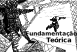
\includegraphics[width=\textwidth]{presentation_sec_one}
\end{frame}

% SUBSEÇÃO
\begin{frame}{Uma Breve Jornada Sobre os Processos}
  \begin{figure}[!h]
    \centering
    \includegraphics[width=.4\textwidth]{memory_segment}
    \caption*{Segmento de memória}
  \end{figure}
\end{frame}

\begin{frame}{Uma Breve Jornada Sobre os Processos}
  \begin{figure}[!h]
    \centering
    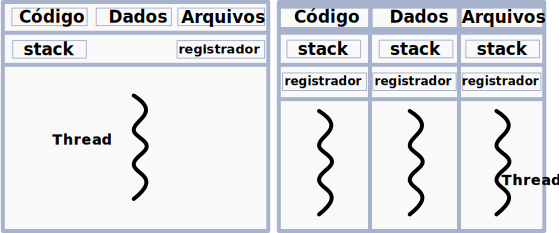
\includegraphics[width=.7\textwidth]{process_and_threads}
    \caption*{Única thread e multi-thread. Note o isolamento da pilha e do registrador (PC)}
    %\caption{Única thread e multi-thread. Note o isolamento da pilha e dos registrador (PC)~\citep{silberschatz}\label{fig:single_thread_multi_thread}}
  \end{figure}
\end{frame}

% SUBSEÇÃO
\begin{frame}[plain]
  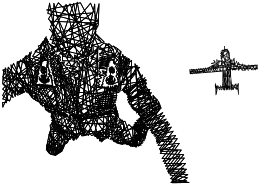
\includegraphics[width=\textwidth]{presentation_sec_two}
\end{frame}

\begin{frame}{Gerenciamento da Memória Relacionada aos Processos}
  \begin{figure}[!h]
    \centering
    \includegraphics[width=.7\textwidth]{virtual_vs_fisico} 
    \caption*{Espaço de endereçamento virtual vs. físico}
  \end{figure}
\end{frame}

%\begin{frame}[plain]
%  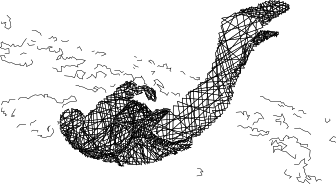
\includegraphics[width=\textwidth]{presentation_sec_four}
%\end{frame}

\begin{frame}{O Modelo de Paginação}
  \begin{figure}[!h]
    \centering
    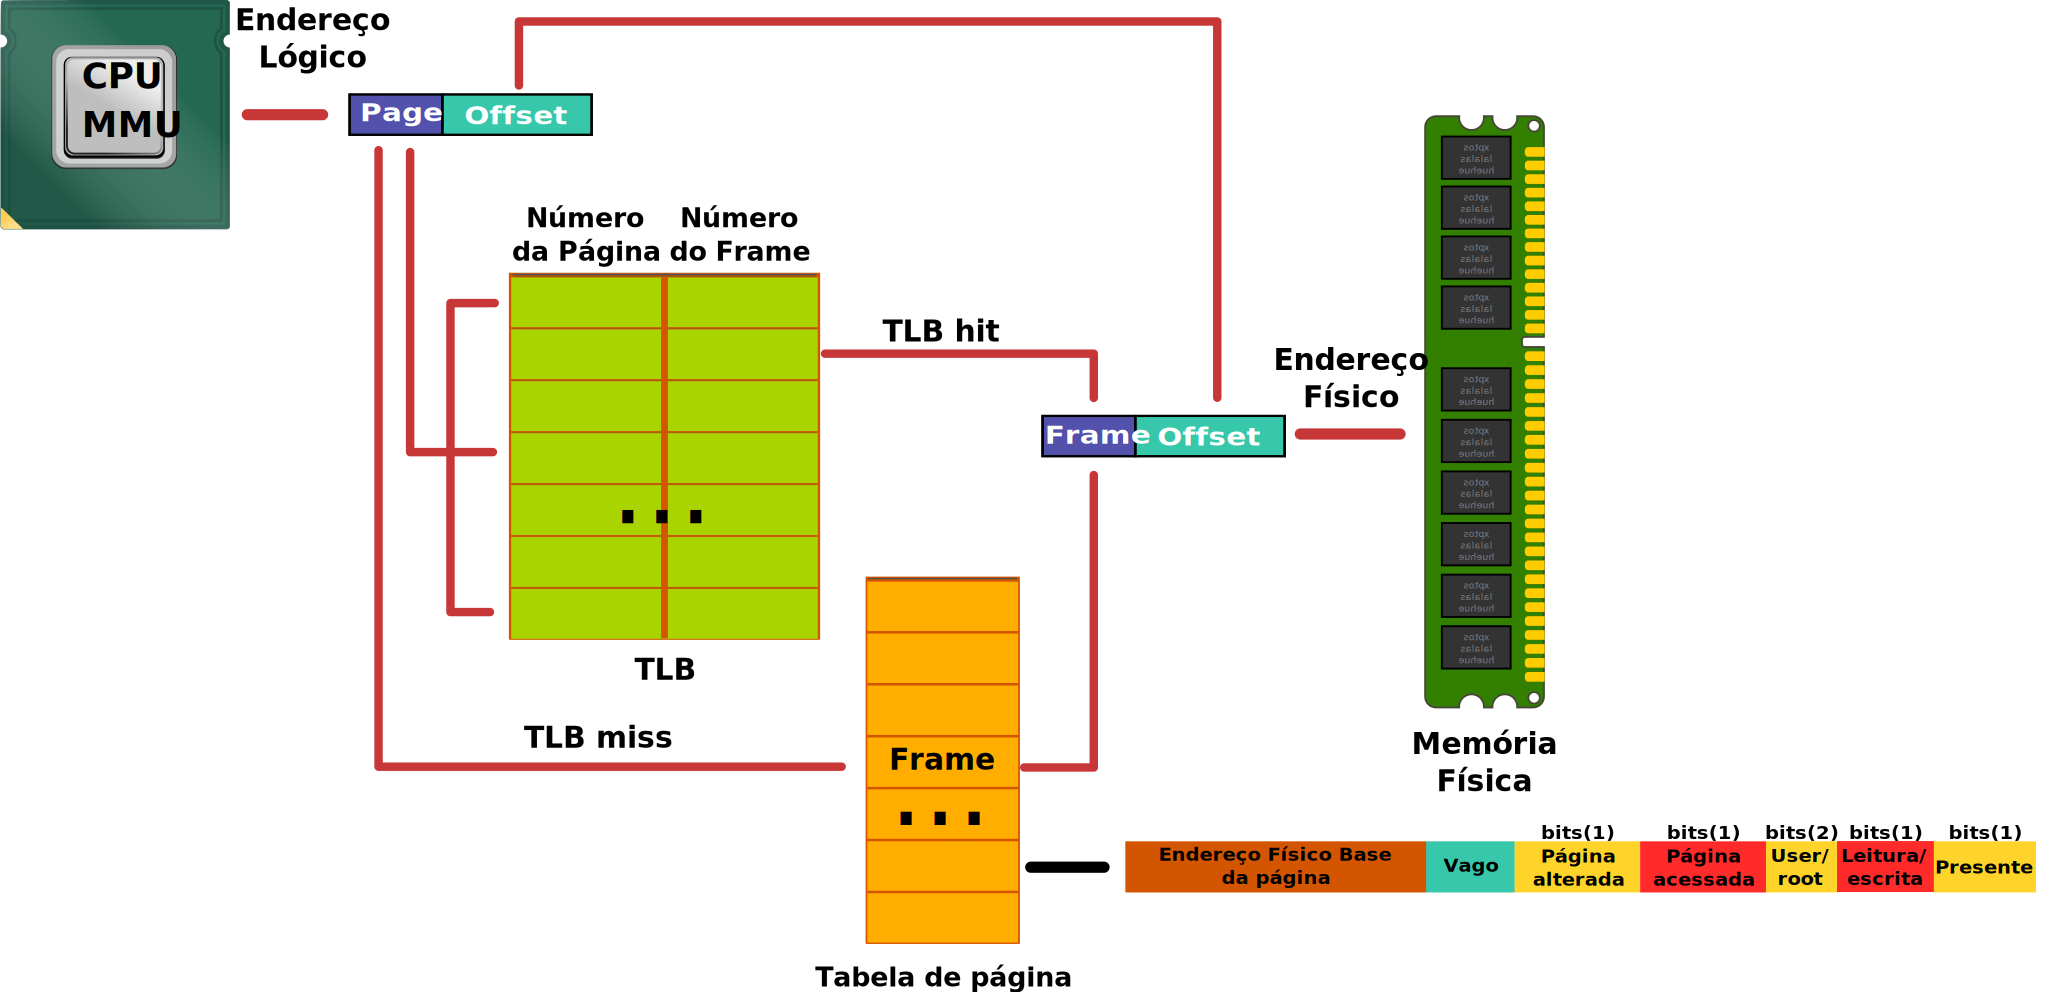
\includegraphics[width=\textwidth]{paginacao_presentation} 
    \caption*{Elementos básicos presentes no modelo de paginação}
  \end{figure}
\end{frame}

%\begin{frame}{Exemplo Prático Usando o GNU/Linux}
%  \begin{figure}[!h]
%    \centering
%    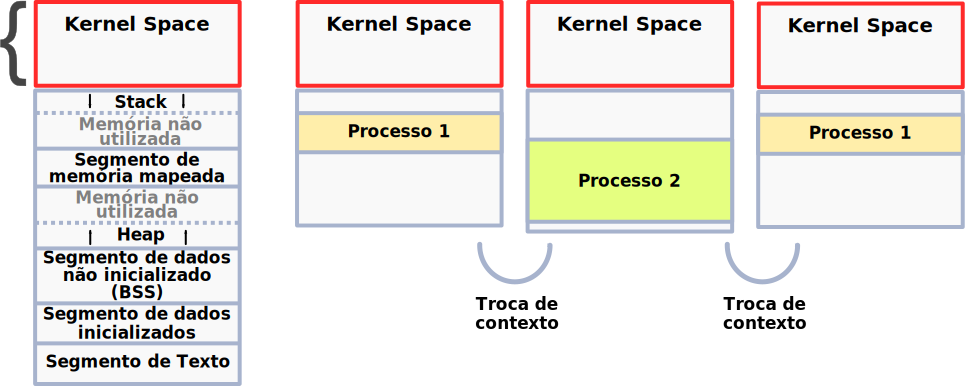
\includegraphics[width=\textwidth]{segmento_troca_contexto}
%    \caption*{VAS durante a troca de contexto}
%    %\caption{VAS durante a troca de contexto~\citep{kernel_manage_mem}}
%  \end{figure}
%\end{frame}

% TODO: MOVER O MALLOC PARA OS RESULTADOS
%
%\begin{frame}[plain]
%  \centering
%  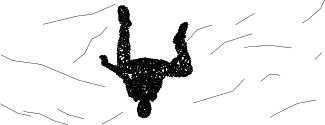
\includegraphics[width=\textwidth]{presentation_sec_nine}
%\end{frame}
%
%\begin{frame}{Exemplo Prático Usando o GNU/Linux}
%  \begin{figure}[!h]
%    \centering
%    \includegraphics[width=\textwidth]{malloc}
%    \caption*{Passos envolvidos na alocação de memória com \texttt{malloc()}}
%    % \caption[Passos envolvidos na alocação de memória com \texttt{malloc()}]{Passos envolvidos na alocação de memória com \texttt{malloc()} (imagem baseada em \cite{anatomy_program_mem})}
%  \end{figure}
%\end{frame}

\begin{frame}[plain]
  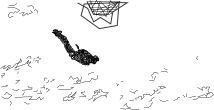
\includegraphics[width=\textwidth]{presentation_sec_five}
\end{frame}

%\begin{frame}[plain]
%  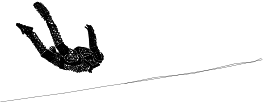
\includegraphics[width=\textwidth]{presentation_sec_six}
%\end{frame}

\begin{frame}{Chamadas de Sistema}
  \begin{figure}[!h]
    \centering
    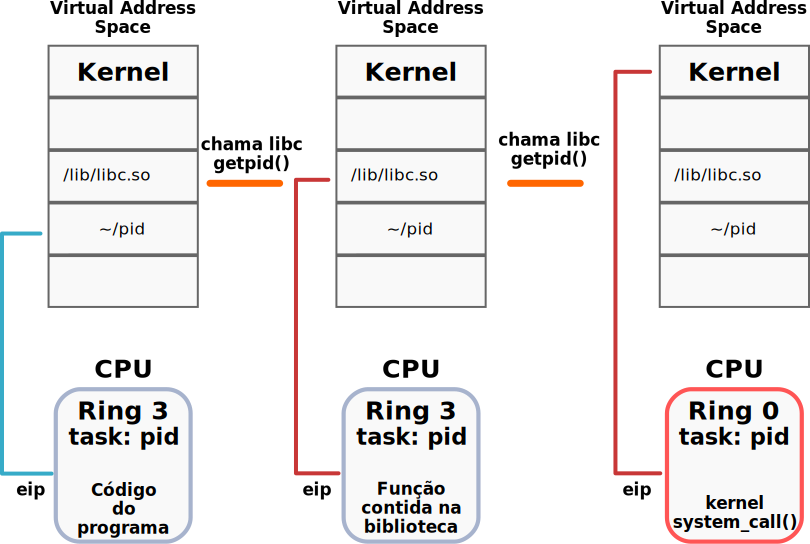
\includegraphics[width=0.5\textwidth]{userspace_to_kernel} 
    \caption*{Execução do user space até o kernel space (\texttt{SYSCALL})}
  \end{figure}
\end{frame}

%\begin{frame}[plain]
%  \centering
%  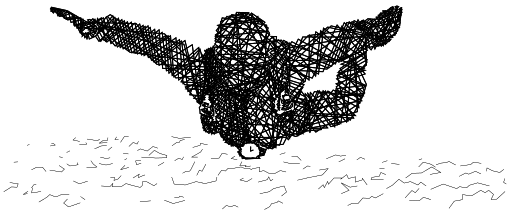
\includegraphics[width=\textwidth]{presentation_sec_eight}
%\end{frame}

%\begin{frame}{Troca de Contexto}
%  \begin{block}{Passos gerais da troca de contexto}
%    \begin{enumerate}
%      \item A troca tem início quando uma interrupção vinda do hardware ocorre
%      \item Salvar o estado do processo em execução
%      \item Carregar o estado do novo processo na CPU
%    \end{enumerate}
%  \end{block}
%\end{frame}

%\begin{frame}{Descritores de Arquivo}
%  \begin{figure}[!h]
%    \centering
%    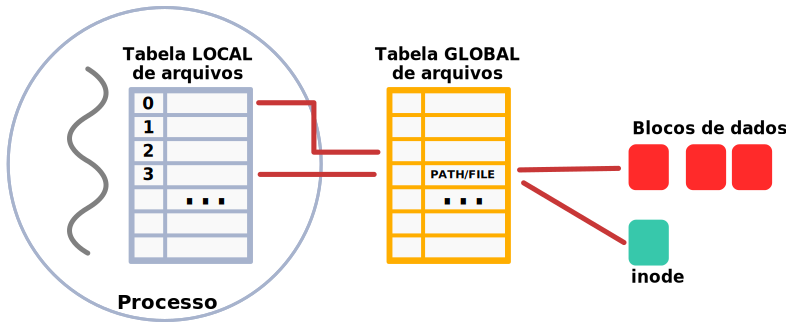
\includegraphics[width=\textwidth]{descritores} 
%    \caption*{Tabela local e global de arquivos}
%  \end{figure}
%\end{frame}
%
%\begin{frame}[plain]
%  \centering
%  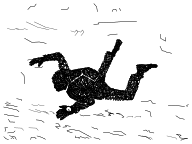
\includegraphics[width=\textwidth]{presentation_sec_seven}
%\end{frame}

\begin{frame}[plain]
  \centering
  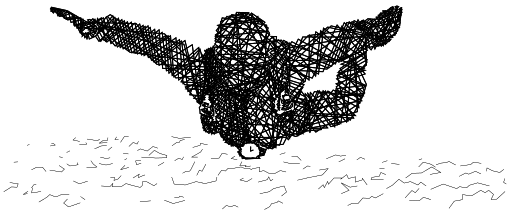
\includegraphics[width=\textwidth]{presentation_sec_eight}
\end{frame}

\begin{frame}{Virtualização}
    \begin{itemize}
      \item \emph{Guest} vs. \emph{Host}
      \item Elemento central da virtualização é o hypervisor, também conhecido
            como Virtual Machine Monitor (VMM)
      \item Virtualização completa em hardware
      \item \texttt{VMCALL}
    \end{itemize}
\end{frame}

\begin{frame}{A Tecnologia VT-x}
  \begin{figure}[!h]
    \centering
    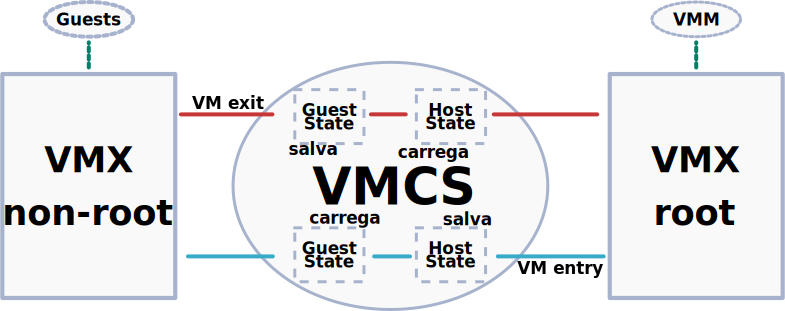
\includegraphics[width=0.7\textwidth]{vt-x_flow} 
    \caption*{Fluxo do comportamento da tecnologia VT-x}
  \end{figure}
\end{frame}

%\begin{frame}[plain]
%  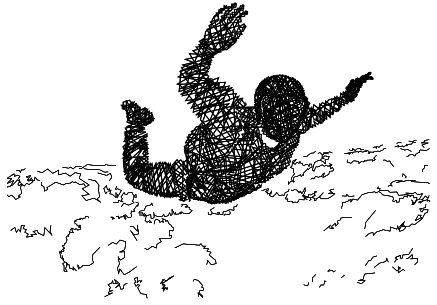
\includegraphics[width=\textwidth]{presentation_sec_three}
%\end{frame}
%
% TODO: MOVER ESSAS PARTES PARA OUTROS LUGARES QUE FAZEM MAIS SENTIDO
%\begin{frame}{Modelos de Programação, Aspectos de Implementação e Gerenciamento de Recursos}
%
%  \begin{proof}[Modelos de Programação]
%    Os SOs fornecem vários recursos adicionais para o espaço de usuário, por
%isso, SOs implementam um dado modelo de programação através de uma API própria
%  \end{proof}
%
%  \begin{proof}[Aspectos de Implementação]
%    As abstrações de processos são o ponto central no projeto de um SO moderno
%de propósito geral, mapeando outras abstrações para ele
%  \end{proof}
%
%  \begin{proof}[Gerenciamento de Recursos]
%    Indiretamente diversos software demandam significativa participação do SO,
%estendendo assim o seu consumo de recursos para o sistema
%  \end{proof}
%
%\end{frame}


%------------------------------------------------------------------------------
% Trabalhos Analisados
%------------------------------------------------------------------------------
\section{Trabalhos Analisados}

\begin{frame}[plain]
  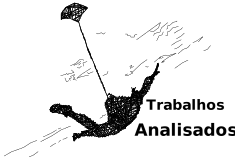
\includegraphics[width=\textwidth]{presentation_cap2_zero}
\end{frame}

\begin{frame}{Dune}

  \begin{proof}[Ideia central]
Utilizar recursos de hardware para virtualização com o objetivo de fornecer
novas características para as abstrações de processos.
  \end{proof}

    \begin{itemize}
      \item Utiliza tecnologia VT-x
      \item Substitui chamadas para \texttt{SYSCALL} por \texttt{VMCALL}
      \item Dune expõe: Exceções, Memória Virtual e Modos privilegiados
      %\item Instruções privilegiadas
      %\item Instruções de controle de fluxo sensíveis
    \end{itemize}

\end{frame}

\begin{frame}{Dune}
  \begin{figure}[!h]
    \centering
    \includegraphics[width=0.4\textwidth]{dune_architecture} 
    \caption*{Arquitetura do Dune}
    %\caption[Arquitetura do Dune]{Arquitetura do Dune~\citep{belay}}
  \end{figure}
\end{frame}

\begin{frame}[plain]
  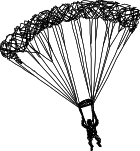
\includegraphics[width=0.5\textwidth]{presentation_cap2_one}
\end{frame}

\begin{frame}{Shreds}

  \begin{proof}[Ideia central]
Evitar abusos intra-processos de conteúdo de memória
  \end{proof}

  \begin{itemize}
    \item Faz uso dos domínios de memória
      \begin{figure}[!h]
        \centering
        
\includegraphics[width=.8\textwidth]{pte_domain} 
        %\caption*{Ilustração de uma entrada da tabela de páginas utilizando novos bits}
      \end{figure}

    \item Fragmento de memória protegida: \emph{shred-private pool (s-pool)}
    \item Pilares do \emph{Shred}: API, \emph{S-compiler} e \emph{S-driver}
  \end{itemize}
\end{frame}

\begin{frame}{Shreds}
  \begin{figure}[!h]
    \centering
    \includegraphics[width=0.6\textwidth]{shreds} 
    \caption*{Funcionamento geral do shreds}
  \end{figure}
\end{frame}

\begin{frame}[plain]
  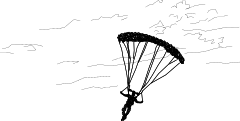
\includegraphics[width=\textwidth]{presentation_cap2_three}
\end{frame}

\begin{frame}{Wedge}

  \begin{proof}[Princípio do Menor Privilégio]

\emph{"O princípio do menor privilégio implica dividir o código em compartimentos,
cada um dos quais executa com os privilégios mínimos necessários para completar
sua tarefa. Essa abordagem não apenas limita o dano que um ataque pode causar,
mas também pode evitar que os \emph{bugs} vazem acidentalmente informações
confidenciais."}% \citep{protectionprinciple}

  \end{proof}

\end{frame}

\begin{frame}{Wedge}
  Primitivas do Wedge: \emph{sthread}, \emph{tagged memory} e \emph{callgates}
  \begin{itemize}
    \item \emph{sthread}: São como \emph{threads}, mas o programador pode atribuir permissões de acesso a memória
    \item \emph{tagged memory}: Contém as permissões de acesso
    \item \emph{callgates}: Uma porção de código que executa em um nível de privilégio diferente de quem o chamou
  \end{itemize}

\end{frame}

%\begin{frame}[plain]
%  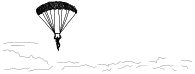
\includegraphics[width=\textwidth]{presentation_cap2_four}
%\end{frame}

\begin{frame}[plain]
  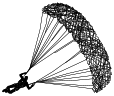
\includegraphics[width=0.7\textwidth]{presentation_cap2_seven}
\end{frame}

\begin{frame}{SpaceJMP}

  \begin{proof}[Ideia central]
Desacoplar o espaço de endereçamento virtual do processo com o objetivo de
permitir mapear memórias na ordem dos petabytes
  \end{proof}

  \begin{figure}[!h]
    \centering
    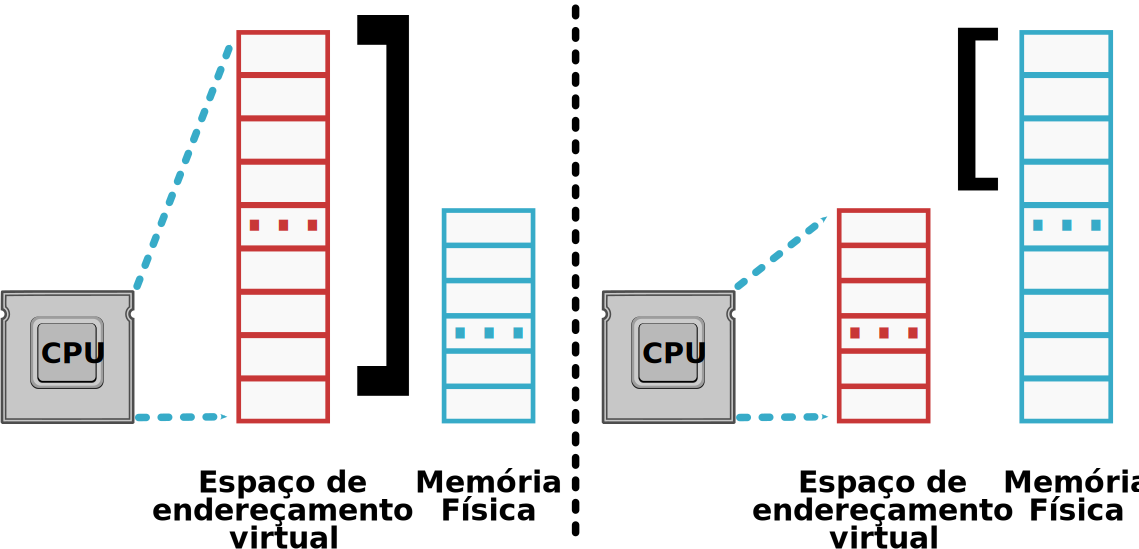
\includegraphics[width=.5\textwidth]{vas_vs_physical_address} 
    \caption*{VAS e Memóra Física}
  \end{figure}

\end{frame}

\begin{frame}{SpaceJMP}
  \begin{figure}[!h]
    \centering
    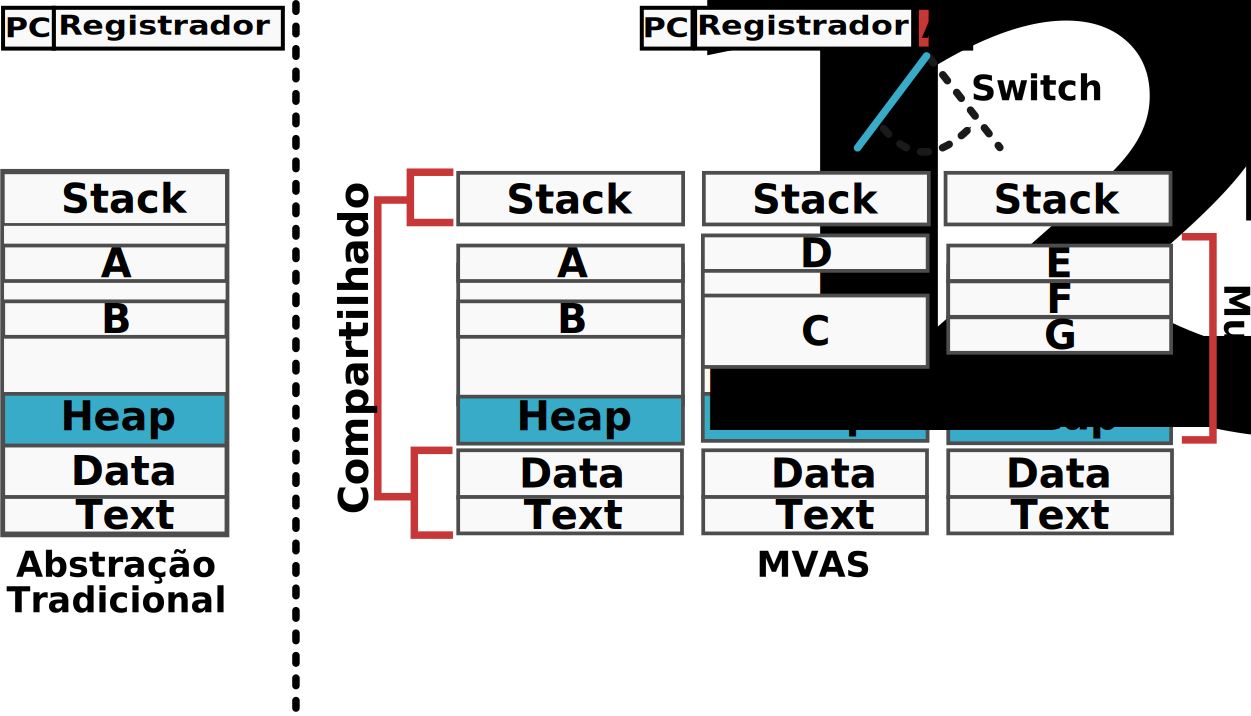
\includegraphics[width=.7\textwidth]{traditional_vs_mvas} 
    \caption*{VAS e MVAS}
    %\caption*{VAS e MVAS \citep{spacejmp}}
  \end{figure}
\end{frame}

\begin{frame}[plain]
  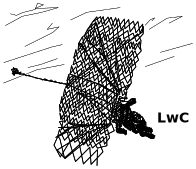
\includegraphics[width=0.7\textwidth]{presentation_cap2_eight}
\end{frame}

\begin{frame}{Light-weight Contexts}

  \begin{proof}[Ideia central]
Desacoplar do isolamento da memória, estado de execução e separação dos
privilégios dos processos trazem benefícios.
  \end{proof}

  \begin{itemize}
    \item Criação de um novo contexto (\texttt{lwCreate})
    \item Troca de contexto (\texttt{lwSwitch})
  \end{itemize}

  \begin{figure}[!h]
    \centering
    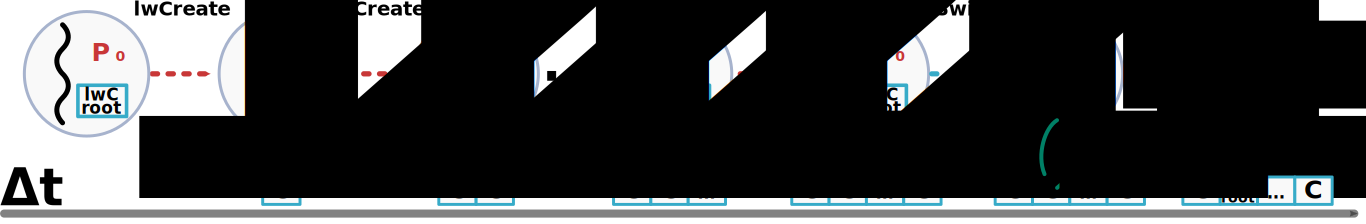
\includegraphics[width=\textwidth]{lwC} 
    \caption*{Exemplo do comportamento do lwC}
  \end{figure}

\end{frame}

%\begin{frame}[plain]
%  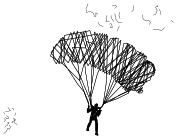
\includegraphics[width=0.7\textwidth]{presentation_cap2_nine}
%\end{frame}

%------------------------------------------------------------------------------
% Validação de Novas Abstrações de Processos
%------------------------------------------------------------------------------
\section{Validação de Novas Abstrações de Processos}

\begin{frame}[plain]
  \includegraphics[width=\textwidth]{presentation_cap3_sec1}
\end{frame}

\begin{frame}{Questões de Pesquisa}
  \begin{quote}
    \item \emph{QP3:.} ``Quais aplicações podem ser utilizadas para avaliar as novas abstrações adicionadas ao SO?''
    \item \emph{QP4:.} ``Qual conjunto de \emph{microbenchmarks} pode ser utilizado para auxiliar a entender os impactos de uma nova característica adicionada às abstrações de processos?''
  \end{quote}
\end{frame}

\begin{frame}{Servidor Apache HTTPD}
  \begin{figure}[!h]
    \centering
    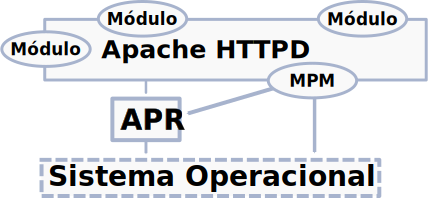
\includegraphics[width=\textwidth]{apache_arhitecture} 
    \caption*{Arquitetura do servidor Apache HTTP}
  \end{figure}
\end{frame}

\begin{frame}{Servidor Apache HTTPD}
  \begin{figure}[!h]
    \centering
    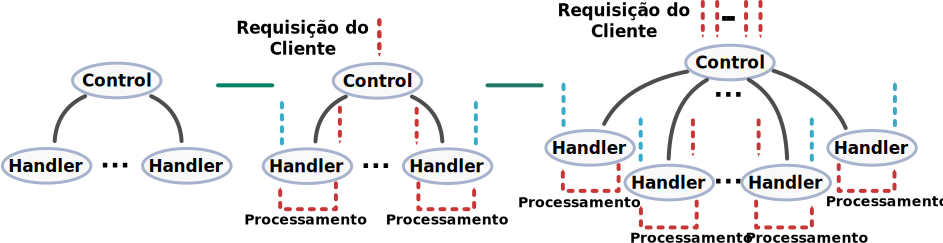
\includegraphics[width=\textwidth]{prefork} 
    \caption*{Prefork}
  \end{figure}
\end{frame}

\begin{frame}{Servidor Apache HTTPD}
  \begin{figure}[!h]
    \centering
    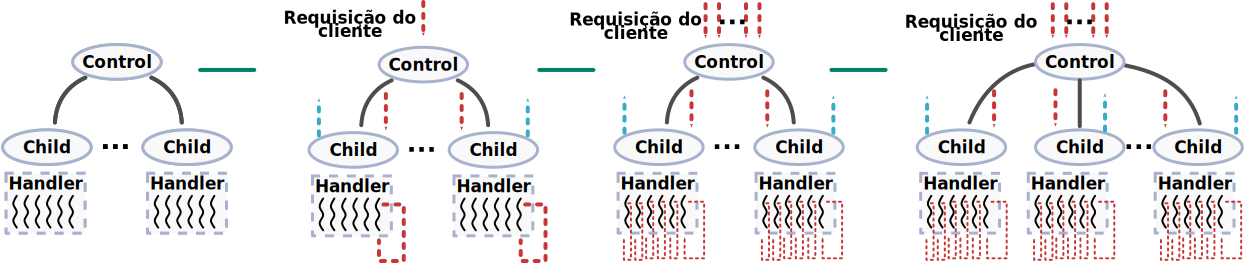
\includegraphics[width=\textwidth]{worker} 
    \caption*{Worker}
  \end{figure}
\addvspace{-20pt}
  \begin{figure}[!h]
    \centering
    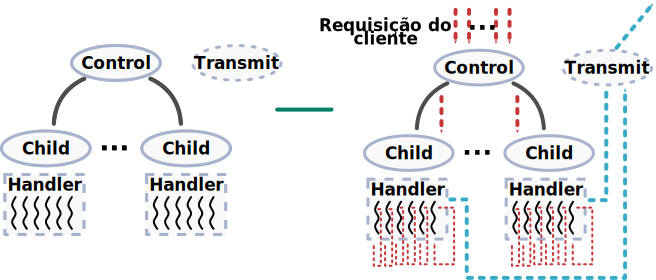
\includegraphics[width=.5\textwidth]{event} 
    \caption*{Event}
  \end{figure}
\end{frame}

\begin{frame}{Nginx}
  \begin{figure}[!h]
    \centering
    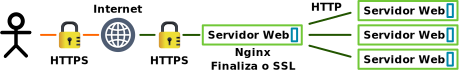
\includegraphics[width=\textwidth]{nginx_load_balancer_ex} 
    \caption*{Nginx comportando-se como reverse-proxy}
    %\caption*[Nginx comportando-se como reverse-proxy]{Nginx comportando-se como reverse-proxy \citep{soni}}
  \end{figure}
\end{frame}

%Ferramentas de Comunicação Criptografada
\begin{frame}[plain]
  \centering
  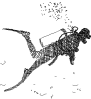
\includegraphics[width=.6\textwidth]{presentation_cap3_sec2}
\end{frame}

\begin{frame}{OpenSSL e OpenSSH}
  \begin{figure}[!h]
    \centering
    \includegraphics[width=\textwidth]{ssl_handshake}
%    \caption*{Do cliente para o servidor Web}
  \end{figure}

  \begin{figure}[!h]
    \centering
    \includegraphics[width=0.4\textwidth]{ssh_layers}
%    \caption*{Camadas SSH}
    %\caption*[Camadas SSH]{Camadas SSH \citep{opensshhood}}
  \end{figure}
\end{frame}

%Outras Aplicações
\begin{frame}[plain]
  \includegraphics[width=.8\textwidth]{presentation_cap3_sec3}
\end{frame}

\begin{frame}{Redis}
  \begin{figure}[!h]
    \centering
    \includegraphics[width=\textwidth]{redis_overview}
    \caption*{Visão geral do funcionamento do Redis}
  \end{figure}
\end{frame}

\begin{frame}{Garbage Collection (GC)}
  \begin{figure}[!h]
    \centering
    \includegraphics[width=\textwidth]{gc_algoritmo}
    \caption*{Algoritmo de pintura da memória}
    %\caption*[Algoritmo de pintura da memória]{Algoritmo de pintura da memória\citep{gc_basics}}
  \end{figure}
\end{frame}

\begin{frame}[plain]
  \centering
  \includegraphics[width=.7\textwidth]{discuss}
\end{frame}

\begin{frame}{Discussão Sobre as Aplicações}
  \begin{table}[]
\small
\centering
  \begin{tabular}{|@{}c@{}|@{}c@{}|@{}c@{}|@{}c@{}|@{}c@{}|@{}c@{}|@{}c@{}|}
  % TOPO DA TABELA
  % |M{2.5cm}|M{2.5cm}|M{2.5cm}|
  \hline
  \multicolumn{1}{|l|}{\diagbox[width=2.5cm, height=2cm]{App}{Alvo}} &
    % Troca de contexto
    \multicolumn{1}{@{}c@{}|}{\begin{tabular}[c]{@{}c@{}}Controle\\fino da\\Memória\end{tabular}} &
    % Persistência de processos
    \multicolumn{1}{@{}c@{}|}{\begin{tabular}[c]{@{}c@{}}Consumo\\ de CPU \end{tabular}} &
    % Controle fino de privilégios
    \multicolumn{1}{@{}c|}{\begin{tabular}[c]{@{}c@{}}Consumo \\de Memória \end{tabular}} &
    % Segurança
    \multicolumn{1}{@{}c|}{Segurança} &
    % Recuperação
    \multicolumn{1}{@{}c|}{Recuperação} &
    % Otimização
    \multicolumn{1}{@{}c|}{Otimização} \\ \hline \hline
  % Início da tabela
  Apache                                                                    & \ding{52}\ding{52}\ding{52} &                    & & & & \ding{52}\ding{52} \\ \hline
  Nginx                                                                   & \ding{52}\ding{52}          & \ding{52}\ding{52} & & & \ding{52}\ding{52} & \\ \hline
  OpenSSL                                                         &                             &                    & & \ding{52} & & \ding{52}\ding{52}\ding{52} \\ \hline
  OpenSSH                                                           & \ding{52}\ding{52}          &                    & \ding{52}\ding{52}\ding{52} & \ding{52}\ding{52} & & \\ \hline
  Redis                                                           &                             &                    & & \ding{52}\ding{52}\ding{52} & \ding{52}\ding{52}\ding{52} & \\ \hline
  GC                                                           &                             &                    & & \ding{52}\ding{52}\ding{52} & \ding{52}\ding{52}\ding{52} & \\ \hline
  \end{tabular}
\caption{Relação aplicações e alvos}
\label{tab:app_alvos}
\end{table}

\end{frame}

%Microbenchmarks
\begin{frame}[plain]
  \includegraphics[width=\textwidth]{presentation_cap3_sec4}
\end{frame}

\begin{frame}{Microbenchmarks}

  \begin{itemize}
    \item Medir tempo gasto com novos mecanismos de alocação de memória
    \item Medir tempo gasto com operações de leitura e escrita
    \item Tempo total gasto na chamada em um contexto de concorrência
    \item Quantidade de trocas de contexto
    \item Custos de operações que executam VM Entry e Exit
    \item Medir o uso de EPT
  \end{itemize}

\end{frame}

%------------------------------------------------------------------------------
% Estudo de caso
%------------------------------------------------------------------------------
\section{Estudo de caso}

\begin{frame}[plain]
  \centering
  \includegraphics[width=\textwidth]{presentation_cap4_sec1}
\end{frame}

\begin{frame}{Metodologia}
  \begin{figure}[!h] \centering
    \includegraphics[width=\textwidth]{experiment_arhitecture}
    \caption*{Arquitetura do experimento}
  \end{figure}
\end{frame}

\begin{frame}{Resultados}
  \begin{figure}[!h]
    \centering
    \includegraphics[width=.8\textwidth]{static_file}
  \end{figure}
\end{frame}

\begin{frame}{Resultados}
  \begin{figure}[!h]
    \centering
    \includegraphics[width=.7\textwidth]{static_file_memory_usage}
  \end{figure}
\end{frame}

\begin{frame}{Resultados}
  \begin{figure}[!h]
    \centering
    \includegraphics[width=.8\textwidth]{dynamic_file_request_time}
  \end{figure}
\end{frame}

\begin{frame}{Resultados}
  \begin{figure}[!h]
    \centering
    \includegraphics[width=.7\textwidth]{dynamic_file_memory_usage}
  \end{figure}
\end{frame}

\begin{frame}[plain]
  \centering
  \includegraphics[width=.7\textwidth]{discuss}
\end{frame}

\begin{frame}{Discussão Sobre os Experimentos}
  \begin{figure}[!h]
    \centering
    \includegraphics[width=\textwidth]{mvas_httpd}
    \caption*{HTTPD com MVAS}
  \end{figure}
  \begin{figure}[!h]
    \centering
    \includegraphics[width=\textwidth]{malloc}
    \caption*{Passos envolvidos na alocação de memória com \texttt{malloc()}}
    % \caption[Passos envolvidos na alocação de memória com \texttt{malloc()}]{Passos envolvidos na alocação de memória com \texttt{malloc()} (imagem baseada em \cite{anatomy_program_mem})}
  \end{figure}
\end{frame}

%------------------------------------------------------------------------------
% Análise Sobre Abstrações de Processos
%------------------------------------------------------------------------------
\section{Análise Sobre Abstrações de Processos}

%Análise Sobre Abstrações de Processos
\begin{frame}[plain]
  \centering
  \includegraphics[width=\textwidth]{presentation_cap7}
\end{frame}

\begin{frame}{Análise Sobre Abstrações de Processos}
  \begin{quote}
   \item \textit{QP1:.} ``Quais são as características desejáveis para a próxima geração de abstrações de processos?''
   \item \textit{QP2:.} ``Quais são os principais desafios em se implementar a próxima geração de abstrações de processos?''
  \end{quote}
\end{frame}

\begin{frame}{Potenciais e Dificuldades Para a Adoção de Novas Abstrações de Processos}
  \begin{table}[]
\small
\centering

\begin{tabular}{|@{}c@{}|@{}c@{}|@{}c@{}|@{}c@{}|@{}c@{}|@{}c@{}|@{}c|c@{}|@{}c@{}|}
% HEADERS
\hline
  \multirow{2}{*}{Trabalho}          &
  \multicolumn{3}{c|}{Dependência}   &
  \multicolumn{2}{c|}{Implementação} &
  \multicolumn{2}{c|}{Hardware}       &
  \multirow{2}{*}{Adoção} \\ \cline{2-8} &
      Técnica & Compatibilidade & Compilador & Pesada & Independente &
      \multicolumn{1}{c|}{Novo} & Característica &
\\ \hline
%           Técnica     Compatib    Compilaca   Pesada      Independente                     Novo        Caracact   Adocao
Dune      & \ding{54} & \ding{54} & \ding{54} & \ding{54} & \multicolumn{1}{c|}{\ding{54}} & \ding{54} & \ding{52} & \\ \hline
Shreds    & \ding{54} & \ding{52} & \ding{52} & \ding{52} & \multicolumn{1}{c|}{\ding{54}} & \ding{54} & \ding{52} & \\ \hline
Wedge     & \ding{54} & \ding{52} & \ding{52} & \ding{52} & \multicolumn{1}{c|}{\ding{54}} & \ding{54} & \ding{54} & \\ \hline
\begin{tabular}[c]{@{}c@{}}Resource\\ Container\end{tabular} & & & & & \multicolumn{1}{c|}{} & & & \\ \hline
Nooks     & \ding{54} & \ding{52} & \ding{54} & \ding{52} & \multicolumn{1}{c|}{\ding{54}} & \ding{54} & \ding{54} & \\ \hline
Mondrian  & -- & -- & -- & -- & \multicolumn{1}{c|}{ -- } & -- & -- & \\ \hline
SpaceJMP  & \ding{54} & \ding{52} & \ding{52} & \ding{52} & \multicolumn{1}{c|}{\ding{54}} & \ding{54} & \ding{54} & \\ \hline
LwC       & \ding{54} & \ding{52} & \ding{54} & \ding{52} & \multicolumn{1}{c|}{\ding{54}} & \ding{54} & \ding{54} & \\ \hline
Exokernel & -- & -- & -- & -- & \multicolumn{1}{c|}{--} & -- & -- & \\ \hline
\end{tabular}

\caption{Potencial de adoção}
\label{tab:adocao}

\end{table}

\end{frame}

\begin{frame}{Extração de Conceitos Derivados das Pesquisas em Abstrações de Processos}
  \begin{itemize}
    \item Dune -- Desacoplamento da virtualização
    \item Nooks e Resource Container -- Desacoplamento do gerenciamento de recursos
    \item SpaceJMP -- Desacoplamento do VAS
    \item Light-weight Context -- Desacoplamento do PC
    \item Wedge -- Desacoplamento de privilégios
    \item Mondrix/Mondrian -- Desacoplamento do controle de memória
  \end{itemize}
\end{frame}

\begin{frame}{Bead: Um Modelo Teórico Para a Próxima Geração de Abstrações de Processos}
  \begin{table}[]
\small
\centering
  \begin{tabular}{|@{}c@{}|@{}c@{}|@{}c@{}|@{}c@{}|@{}c@{}|@{}c@{}|@{}c@{}|}
  % TOPO DA TABELA
  % |M{2.5cm}|M{2.5cm}|M{2.5cm}|
  \hline
  \multicolumn{1}{|l|}{\diagbox[width=2.5cm, height=2cm]{Desacoplar}{Vantagem}} &
    % Troca de contexto
    \multicolumn{1}{@{}c@{}|}{\begin{tabular}[c]{@{}c@{}}Novos\\modelos de\\programação\end{tabular}} &
    % Persistência de processos
    \multicolumn{1}{@{}c@{}|}{\begin{tabular}[c]{@{}c@{}} Persistência\\ de processos \end{tabular}} &
    % Controle fino de privilégios
    \multicolumn{1}{@{}c|}{\begin{tabular}[c]{@{}c@{}}Controle \\fino de \\ privilégios\end{tabular}} &
    % Segurança
    \multicolumn{1}{@{}c|}{Segurança} &
    % Recuperação
    \multicolumn{1}{@{}c|}{Recuperação} &
    % Otimização
    \multicolumn{1}{@{}c|}{Otimização} \\ \hline \hline
  % Início da tabela
  PC                                                                    & \ding{52}\ding{52}\ding{52} &                    & & & & \ding{52}\ding{52} \\ \hline
  VAS                                                                   & \ding{52}\ding{52}          & \ding{52}\ding{52} & & & \ding{52}\ding{52} & \\ \hline
  \begin{tabular}[c]{@{}c}Resource\\ Management\end{tabular}            & \ding{52}                   &                    & & & \ding{52}\ding{52}\ding{52} & \ding{52} \\ \hline
  \begin{tabular}[c]{@{}c}Controle de\\ acesso a\\ memória\end{tabular} &                             &                    & \ding{52}\ding{52}\ding{52} & \ding{52}\ding{52} & & \\ \hline
  Virtualização                                                         &                             &                    & & \ding{52} & & \ding{52}\ding{52}\ding{52} \\ \hline
  Privilégios                                                           & \ding{52}\ding{52}          &                    & \ding{52}\ding{52}\ding{52} & \ding{52}\ding{52} & & \\ \hline
  Comunicação                                                           &                             &                    & & \ding{52}\ding{52}\ding{52} & \ding{52}\ding{52}\ding{52} & \\ \hline
  \end{tabular}
\caption{Relação desacoplamento benefício}
\label{tab:desacoplamento_beneficio}
\end{table}

\end{frame}

\begin{frame}{Bead: Um Modelo Teórico Para a Próxima Geração de Abstrações de Processos}
  \begin{figure}[!h]
    \centering
    \includegraphics[width=\textwidth]{decomposicao_overview}
    \caption*{Decomposição do processo}
  \end{figure}
\end{frame}

\begin{frame}{A API Bead}
  \begin{columns}[t]
    \col
      \begin{itemize}
        \item \texttt{BEAD\_SET\_CONFIG}
        \item \texttt{BEAD\_GET\_CONFIG}
        \item \texttt{BEAD\_NEW\_CONTEXT\_INSTANCE}
        \item \texttt{BEAD\_SWITCH}
        \item \texttt{BEAD\_VIRTUALIZATION\_MODE}
      \end{itemize}
    \col
      \begin{itemize}
        \item \texttt{BEAD\_ENTER\_COMPARTMENT}
        \item \texttt{BEAD\_EXIT\_COMPARTMENT}
        \item \texttt{BEAD\_ALLOC\_COMPARTMENT}
        \item \texttt{BEAD\_FREE\_COMPARTMENT}
      \end{itemize}
  \end{columns}
\end{frame}

\begin{frame}{Padrões de Utilização}
  \begin{columns}[t]
    \col
      \centering
      \includegraphics[width=0.8\textwidth]{beadctlOne}
    \col
      \centering
      \includegraphics[width=0.7\textwidth]{beadctlTwo}
  \end{columns}
 %\begin{pseudocode}

\begin{lstlisting}[language=pseudocode, style=pseudocode]
function beadctl(code, data)
  ret $\gets 0$
  switch(code)
    case BEAD_SET_CONFIG:
      ret $\gets$ \func{bead_set_config(data)}
      break
    case BEAD_GET_CONFIG:
      ret $\gets$ \func{bead_get_config(data)}
      break
    case BEAD_NEW_CONTEXT_INSTANCE:
      ret $\gets$ \func{bead_ctx_instance(data)}
      break
    case BEAD_SWITCH:
      ret $\gets$ \func{bead_ctx_switch(data)}
      break
    case BEAD_VIRTUALIZATION_MODE:
      ret $\gets$ \func{bead_virtualization(data)}
      break
    case BEAD_ALLOC_COMPARTMENT:
      /// ...
    case BEAD_FREE_COMPARTMENT:
      /// ...
    case BEAD_ENTER_COMPARTMENT:
      break
      /// ...
    case BEAD_EXIT_COMPARTMENT:
      /// ...
    default:
      /// ...

  return ret

\end{lstlisting}

  \caption{Função de controle das propriedades do \emph{bead}}
  \label{alg:ctlbead}
\end{pseudocode}

 %\begin{pseudocode}

\begin{lstlisting}[language=pseudocode, style=pseudocode]
struct bead_data {
  ENABLE_RECURSIVE_SNAPSHOT, // Total de fotografias recursivas, falso por padrão
  MAX_SNAPSHOT_LEVEL, // Total de fotografias recursivas
  TOTAL_OF_SNAPSHOT, // Total de fotografias tiradas
  CTX_IDS[], // Estrutura de dados contendo as referências para os ids
  VITUALIZATION_FLAGS, // Conjunto de flags de controle sobre quais recursos oferecer para o processo
  VAS_FLAGS, // Conjunto de flags utilizada para controlar o desacoplamento da VAS
  SWITCH_OPTION, // 
}

\end{lstlisting}

  \label{alg:beadata}
  \caption{Estrutura de dados utilizada pelo bead para troca de dados do espaço de usuário com o de kernel (vice-versa)}
\end{pseudocode}

\end{frame}

\begin{frame}{Padrão Configuração}
  \begin{figure}[!h]
    \centering
    \includegraphics[width=\textwidth]{decomposition_conf}
    \caption*{Ilustração do padrão configuração}
  \end{figure}
\end{frame}

\begin{frame}{Padrão Configuração}
  \centering
  \includegraphics[width=\textwidth]{padraoConfig}
\end{frame}

\begin{frame}{Padrão Fotografia}
  \begin{figure}[!h]
    \centering
    \includegraphics[width=\textwidth]{decomposition_fotografia}
    \caption*{Ilustração dos principais elemento envolvidos no padrão fotografia}
  \end{figure}
\end{frame}

\begin{frame}{Padrão Virtualização Controlada}
  \begin{figure}[!h]
    \centering
    \includegraphics[width=.8\textwidth]{decomposicao_virt_controlada}
    \caption*{Ilustração dos elementos envolvidos no padrão virtualização}
  \end{figure}
\end{frame}

\begin{frame}{Padrão Atualização em Tempo Real}
  \begin{figure}[!h]
    \centering
    \includegraphics[width=\textwidth]{live-patching}
    \caption*{Funcionamento do padrão atualização em tempo real}
  \end{figure}
\end{frame}

%------------------------------------------------------------------------------
% Conclusão
%------------------------------------------------------------------------------
\section{Conclusão}

%Conclusão
\begin{frame}[plain]
  \includegraphics[width=.9\textwidth]{self-made}
\end{frame}

\begin{frame}{Conclusão}
  \begin{itemize}
    \item Estabelecemos um panorama sobre diversos trabalhos relacionados a
          abstração de processos
    \item Formas de validação
    \item Uma visão para a nova geração de abstrações de processos
  \end{itemize}
\end{frame}

\begin{frame}{Trabalhos Futuros}
  \begin{itemize}
    \item Survey sobre abstrações de processos
    \item Ferramenta de testes para as novas abstrações
    \item Implementar o bead no Linux
  \end{itemize}
\end{frame}

%------------------------------------------------------------------------------
% Perguntas
%------------------------------------------------------------------------------
\begin{frame}{Perguntas}
  \tableofcontents
\end{frame}

\appendix

\begin{frame}{Servidores Web}
  \begin{figure}[!h]
    \centering
    \includegraphics[width=.8\textwidth]{request_a_page}
    \caption*{Do cliente para o servidor Web.}
  \end{figure}
\end{frame}

\begin{frame}{Servidores Web}
  \begin{figure}[!h]
    \centering
    \includegraphics[width=\textwidth]{with_without_keep_alive}
  \end{figure}
\end{frame}

\begin{frame}{O Modelo de Paginação}
  \begin{figure}[!h]
    \centering
    \includegraphics[width=0.6\textwidth]{paginacao_passos} 
    \caption*{Passos do acesso a memória usando o modelo de paginação. A figura ilustra o caso simples na qual pelo menos dois acessos a memória são necessários}
  \end{figure}
\end{frame}

\begin{frame}{Nooks}
  \begin{proof}[Ideia central]
Nooks é uma camada que se interpõe entre o Kernel e suas extensões. Essa camada
comporta-se como um subsistema responsável por tratar as operações passadas via
kernel para os módulos e vice-versa; o controle feito sobre cada parte
representa uma camada a mais de verificação que adiciona mais segurança e
confiabilidade para o SO.
  \end{proof}
\end{frame}

\begin{frame}{SpaceJMP}
  \begin{figure}[!h]
    \centering
    \includegraphics[width=.7\textwidth]{solve_huge_address_memory}
    \caption*{Resolvendo o problema de endereçar memórias físicas grandes}
  \end{figure}
\end{frame}

\begin{frame}{Customizações no Servidor Apache e no GNU/Linux}
  \begin{table}
  \centering
  \begin{tabular}{|c|c|c|c|}
  \hline
    \textit{Parameter} & \textbf{Event} & \textbf{Worker} & \textbf{Prefork} \\
      \hline\hline
    \textbf{ServerLimit} & 6000 & 6000 & 5000\\
      \hline
    \textbf{StartServer} & 10 & 10 & 1000\\
      \hline
    \textbf{MinSpareThreads} & 512 & 512 & --\\
      \hline
    \textbf{MaxSpareThreads} & 1024 & 1024 & --\\
      \hline
    \textbf{ThreadLimit} & 64 & 64 & --\\
      \hline
    \textbf{ThreadPerChild} & 64 & 64 & --\\
      \hline
    \textbf{MaxRequestWorkers} & 5120 & 5120 & 5000\\
      \hline
    \textbf{MinSpareServers} & -- & -- & 500\\
      \hline
    \textbf{MaxSpareServers} & -- & -- & 1500\\
      \hline
  \end{tabular}

  \caption{Configuração adotada para o MPM}
  \label{tab:configuration}

\end{table}


\end{frame}

\begin{frame}{Customizações no Servidor Apache e no GNU/Linux}
  \begin{table}
  \centering
  \begin{tabular}{|c|c|} \hline
  \textit{parameter} & \textbf{value}\\
    \hline\hline
   Max queue events & 1048576\\
     \hline
   Max user instances & 1048576\\
    \hline
   Max user watches & 1048576\\
    \hline
   Max map count & 262144\\
    \hline
   TCP max syn backlog & 8096\\
    \hline TCP syncookies & 0\\
    \hline
  \end{tabular}

  \caption{Configurações feitas no Kernel}
  \label{tab:kernel_config}
\end{table}


\end{frame}

\begin{frame}{Discussão}
  \begin{itemize}
    \item Dependência Técnica
    \item Dependência de Compatibilidade
    \item Dependência de Compilador
    \item Implementação Pesada
    \item Implementação Independente
    \item Hardware Novo
    \item Característica Específica de Hardware
  \end{itemize}
\end{frame}

\begin{frame}{Padrões de Utilização}
  \centering
  \includegraphics[width=\textwidth]{beadData}
\end{frame}

\begin{frame}{Exemplo Prático Usando o GNU/Linux}
  \begin{figure}[!h]
    \centering
    \includegraphics[width=.9\textwidth]{kernel_manages_memory}
    \caption*{Visão interna do gerenciamento da memória}
  \end{figure}
\end{frame}

\begin{frame}{Virtualização}
    \begin{itemize}
      \item \emph{Guest} vs. \emph{Host}
      \item Elemento central da virtualização é o hypervisor, também conhecido
            como Virtual Machine Monitor (VMM)
      \item Virtualização completa em hardware
          \begin{itemize}
          \item Instruções sensíveis
          \item Instruções privilegiadas
          \item Instruções de controle de fluxo sensíveis
      \end{itemize}
      \item \texttt{VMCALL}
    \end{itemize}
\end{frame}

\begin{frame}{O Modelo de Segmentação}
  \begin{figure}[!h]
    \centering
    \includegraphics[width=.80\textwidth]{segmentacao} 
    \caption*{Comportamento do modelo de segmentação. Note que a tabela de segmento é acessada para obter o valor base e esse é sempre verificado para evitar acessos indevidos a outras regiões da memória}
  \end{figure}
\end{frame}

\begin{frame}{SpaceJMP}
  \begin{figure}[!h]
    \centering
    \includegraphics[width=.7\textwidth]{mvas_example} 
    \caption*{System Call disponibilizada pelo SpaceJMP}
    %\caption*{System Call disponibilizada pelo SpaceJMP \cite{ellarge}}
  \end{figure}
\end{frame}

\begin{frame}{Servidor Apache HTTPD}
  \begin{figure}[!h]
    \centering
    \includegraphics[width=\textwidth]{request_phases} 
    \caption*{Gerador de Conteúdo}
    %\caption*[Gerador de Conteúdo]{Gerador de Conteúdo \citep{apache_module_book}}
  \end{figure}
\end{frame}

\begin{frame}{Metodologia}
  \begin{figure}[!h] \centering
    \includegraphics[width=\textwidth]{web_server_organization_strategy}
    \caption*{Visão geral da organização de aplicações utilizando servidores Web}
  \end{figure}
\end{frame}

\begin{frame}{Garbage Collection (GC)}
  \begin{figure}[!h]
    \centering
    \includegraphics[width=\textwidth]{gc_memory}
    \caption*{Visão da memória durante a aplicação do algoritmo de GC}
    %\caption*[Visão da memória durante a aplicação do algoritmo de GC]{Visão da memória durante a aplicação do algoritmo de GC\citep{gc_basics}}
  \end{figure}
\end{frame}

\begin{frame}{Microbenchmarks}
  \begin{proof}[Microbenchmarks]
Microbenchmarks têm por objetivo mensurar e fornecer meios para analisar uma
única característica do objeto de estudo. Eles facilitam o processo de
desenvolvimento, mostram o impacto em um único elemento de forma a facilitar a
análise e são relativamente simples de serem implementados.
  \end{proof}
\end{frame}

\begin{frame}{Device Drivers}
  \begin{figure}[!h]
    \centering
    \includegraphics[width=0.3\textwidth]{dd} 
    \caption*{Tabela local e global de arquivos}
  \end{figure}
\end{frame}

\begin{frame}{Uma Breve Jornada Sobre os Processos}
  \begin{figure}[!h]
    \centering
    \includegraphics[width=\textwidth]{stack_frame}
    \caption*{Alocação e desalocação de Stack frames considerando o padrão CDECL}
    %\caption{Alocação e desalocação de Stack frames considerando o padrão CDECL~\citep{patterson}\label{fig:stack_frames}}
  \end{figure}
\end{frame}

\begin{frame}{OpenSSL}
  \begin{figure}[!h]
    \centering
    \includegraphics[width=\textwidth]{openssl_arch}
    \caption*{Arquitetura do OpenSSL}
  \end{figure}
\end{frame}

\begin{frame}{Cenário}
  \begin{table}[!h]
  \centering
  \begin{tabular}{|c|c|c|}
      \hline 
    & \textbf{Pequeno} & \textbf{Grande}\\
      \hline\hline
    Static & 70Kb & 120Kb\\
      \hline
    Dynamic & 80Kb & 120Kb \\
      \hline
  \end{tabular}

  \caption{Tamanho dos arquivos para serem transferidos}
  \label{tab:file_size}
\end{table}


  \begin{table}[h!]
  \centering
  \begin{tabular}{|c|c|c|}
      \hline
    Casos & \textbf{Requisições} & \textbf{Concorrência}\\
      \hline\hline
    Arquivos estáticos & 60000 & 20000\\
      \hline
    Arquivos dinâmicos & 5000 & 600 \\
      \hline
  \end{tabular}
  \caption{Carga principal aplicada}
  \label{tab:loads}
\end{table}


\end{frame}

\begin{frame}{MVAS Dentro do GNU/Linux e Apache HTTP Server}
  \begin{table}[h!]
  \centering
  \begin{tabular}{|c|c|c|}
      \hline
    Nome & \textbf{Núcleo} & \textbf{Memória}\\
      \hline
    M1 & 2 & 13Gb \\
      \hline
    M2 & 2 & 4Gb \\
      \hline
   \end{tabular}

  \caption{Hardware}
  \label{tab:machines}
\end{table}


\end{frame}

\begin{frame}{Padrão Persistência}
  \begin{figure}[!h]
    \centering
    \includegraphics[width=.4\textwidth]{persistente}
  \end{figure}
\end{frame}

\begin{frame}{Padrão Compartimento}
  %\begin{pseudocode}
\begin{lstlisting}[language=pseudocode, style=pseudocode]
function special_function() /// \label{line:compartimentoFuncaoEsp}
  struct bead_data bead

  bead.compartment_size $\gets 300$
  \func{beadctl(BEAD_SET_CONFIG, &bead)}
  // ... qualquer código que precisa de um bom isolamento ...
  // Aloca memória dentro do compartimento
  \func{beadctl(BEAD_ALLOC_COMPARTMENT_MEMORY, &bead)} /// \label{line:compartimentoAlloc}
  // Libera a memória do compartimento
  \func{beadctl(BEAD_FREE_COMPARTMENT_MEMORY, &bead)} /// \label{line:compartimentoFree}

function enter_compartment()
  struct bead_data bead

  bead.compartments $\gets$ BEAD_ENTER_COMPARTMENT /// \label{line:compartimentoConfig}
  \func{beadctl(BEAD_SET_CONFIG, &bead)}
  \func{beadctl(BEAD_SWITCH, &bead)} // Troca o contexto de executação atual

function exit_compartment() /// \label{line:compartimentoExit}
  struct bead_data bead

  bead.compartments $\gets$ BEAD_EXIT_COMPARTMENT
  \func{beadctl(BEAD_SET_CONFIG, &bead)}
  \func{beadctl(BEAD_SWITCH, &bead)} // Troca o contexto de executação atual

function MAIN() /// \label{line:compartimentoMAIN}
  // ... qualquer código ...
  // Função crítica
  \func{enter_compartment()} /// \label{line:compartimentoEnter}
  \func{special_function()}
  \func{exit_compartment()}
  // ... qualquer código ...
  
\end{lstlisting}

  \caption{Padrão compartimento}
  \label{alg:compartimento}
\end{pseudocode}

  \begin{columns}[t]
    \col
      \centering
      \includegraphics[width=0.8\textwidth]{compartimentoOne}
    \col
      \centering
      \includegraphics[width=0.8\textwidth]{compartimentoTwo}
  \end{columns}
\end{frame}

\begin{frame}{Resource Container}

  \begin{proof}[Ideia central]
Criação de uma entidade lógica que contém os recursos utilizados pelas aplicações.
  \end{proof}

  \begin{figure}[!h]
    \centering
    \includegraphics[width=.8\textwidth]{resource_constainer_scenarios} 
    \caption*{Cenários das aplicações}
  \end{figure}
%    \begin{itemize}
%      \item Fornece mecanismos para ligar recursos a uma \emph{thread}
%      \item Operações para \emph{Resource Container}
%    \end{itemize}

\end{frame}

\begin{frame}[plain]
  \includegraphics[width=\textwidth]{presentation_cap2_five}
\end{frame}

\begin{frame}{Nooks}
  \begin{figure}[!h]
    \centering
    \includegraphics[width=0.8\textwidth]{nooks_nim}
    \caption*{Visão geral da arquitetura do Nooks}
    %\caption*[Visão geral da arquitetura do Nooks]{Visão geral da arquitetura do Nooks \citep{nooks}}
  \end{figure}
\end{frame}

\begin{frame}{Nooks}
  \begin{figure}[!h]
    \centering
    \includegraphics[width=0.8\textwidth]{nooks_mem}
    \caption*{Acesso à memória do Nooks}
    %\caption*[Acesso à memória do Nooks]{Acesso à memória do Nooks \citep{nooks}}
  \end{figure}
\end{frame}

\begin{frame}[plain]
  \includegraphics[width=0.7\textwidth]{presentation_cap2_six}
\end{frame}

\begin{frame}{Mondrian Memory Protection e Mondrix}

  \begin{proof}[Ideia central]
Buscaram explorar técnicas para realizar controle fino sobre da memória, com o
objetivo de adicionar mais confiabilidade e segurança para os SOs.
  \end{proof}

  \begin{itemize}
    \item Solução de hardware: \emph{Mondrian Memory Protection (MMP)}
    \item Solução de software: \emph{Mondrix}
  \end{itemize}

\end{frame}


\begin{frame}{Mondrian Memory Protection e Mondrix}
  \begin{figure}[!h]
    \centering
    \includegraphics[width=0.7\textwidth]{mondrix_pd}
    \caption*{Representação dos domínios de proteção do Mondrix}
    %\caption*{Representação dos domínios de proteção do Mondrix (\cite{mondrix})}
  \end{figure}
\end{frame}


\begin{frame}[t]{Padrão Fotografia}
  \begin{columns}
    \col
      \centering
      \includegraphics[width=0.8\textwidth]{snapshotOne}
    \col
      \centering
      \includegraphics[width=0.9\textwidth]{snapshotTwo}
  \end{columns}
\end{frame}

\begin{frame}{Padrão Virtualização Controlada}
  \begin{columns}[t]
    \col
      \centering
      \includegraphics[width=0.8\textwidth]{virtOne}
    \col
      \centering
      \includegraphics[width=0.8\textwidth]{virtTwo}
  \end{columns}
\end{frame}

\begin{frame}{Padrão Atualização em Tempo Real}
  \begin{figure}[!h]
    \centering
    \includegraphics[width=.4\textwidth]{tempoReal}
  \end{figure}
\end{frame}

\begin{frame}{Exokernel}
  \begin{proof}[Ideia central]
Exokernel busca ser um núcleo mínimo que permita multiplexar de forma segura os
recursos de hardware e ao mesmo tempo fornecer uma interface de baixo-nível na
qual as abstrações do SO podem ser construída sobre ela.
  \end{proof}

  \begin{itemize}
    \item Expor o hardware de forma segura
    \item Expor alocações
    \item Expor nomes
    \item Expor revogações
  \end{itemize}

\end{frame}



\end{document}
